\renewcommand{\thefootnote}{\fnsymbol{footnote}}

\chapter[Introduction to exchange economies]%
 {Introduction to exchange economies}%
\label{ch:L6}

% 3) Reset things so later footnotes go back to 1, 2, 3, …
%\setcounter{footnote}{0}
\renewcommand{\thefootnote}{\arabic{footnote}}

\section{A primer on consumer choice}\label{sec:L6-cons}

Before going to general equilibrium, we need to review some basic concepts on consumer choice. The setting is quite intuitive. There is a single individual \( i \) who can consume a bundle of \( \ell \) different goods. The quantity of each good is represented by a real number. The consumption space is therefore \( \mathbb{R}^{\ell}_+ \). A generic consumption bundle of individual \( i \) is \( x_i = (x^1, \dots, x^{\ell}) \). As an example, if \( \ell = 2 \), a consumption bundle could be \( x_i = (3,5) \), meaning 3 units of good 1 and 5 units of good 2, as represented in Figure~\ref{fig:L6-cons-bundle}. We index consumption bundles by \( i \) because later we will consider multiple individuals, each with his own consumption bundle.

\begin{figure}[H]
    \begin{center}
        \begin{tikzpicture}[x=0.70pt,y=0.70pt,yscale=-1,xscale=1]
            %uncomment if require: \path (0,385); %set diagram left start at 0, and has height of 385

            %Shape: Axis 2D [id:dp11721225431880233] 
            \draw  (135,317.12) -- (483,317.12)(169.8,23) -- (169.8,349.8) (476,312.12) -- (483,317.12) -- (476,322.12) (164.8,30) -- (169.8,23) -- (174.8,30)  ;
            %Shape: Circle [id:dp8937450517881602] 
            \draw  [fill={rgb, 255:red, 0; green, 0; blue, 0 }  ,fill opacity=1 ] (286.4,117.6) .. controls (286.4,115.94) and (287.74,114.6) .. (289.4,114.6) .. controls (291.06,114.6) and (292.4,115.94) .. (292.4,117.6) .. controls (292.4,119.26) and (291.06,120.6) .. (289.4,120.6) .. controls (287.74,120.6) and (286.4,119.26) .. (286.4,117.6) -- cycle ;
            %Straight Lines [id:da41961426078046393] 
            \draw  [dash pattern={on 4.5pt off 4.5pt}]  (289.4,117.6) -- (290,317.6) ;
            %Straight Lines [id:da9291508071819727] 
            \draw  [dash pattern={on 4.5pt off 4.5pt}]  (170,116.6) -- (289.4,117.6) ;

            % Text Node
            \draw (473,329.4) node [anchor=north west][inner sep=0.75pt]    {$x^{1}$};
            % Text Node
            \draw (130,17.4) node [anchor=north west][inner sep=0.75pt]    {$x^{2}$};
            % Text Node
            \draw (285,321.4) node [anchor=north west][inner sep=0.75pt]    {$3$};
            % Text Node
            \draw (154,110.4) node [anchor=north west][inner sep=0.75pt]    {$5$};
        \end{tikzpicture}
        \caption{A consumption bundle \( x_i = (3,5) \) in a two-good consumption space.}
        \label{fig:L6-cons-bundle}
    \end{center}
\end{figure}

Now, say that there is a vector of prices \( p = (p^1, \dots, p^{\ell}) \), where \( p^{\ell} \) is the price of good \( \ell \). Also, assume the individual has monetary wealth \( w_i \in \mathbb{R}_{+} \). He can therefore consume any budle of goods \( x_i \) such that the total expenditure does not exceed his wealth, i.e., such that \( p \cdot x_i \leq w_i \).\footnote{The operation \( \cdot \) denotes the product \( p^{1} \cdot x^1_i + \dots + p^{\ell} \cdot x_i^{\ell} \).} The set of all consumption bundles that satisfy this condition is called the \textbf{budget set}, and is denoted with

\[ B(p,w_i) = \{ x_i \in \mathbb{R}^{\ell}_+ : p \cdot x_i \leq w_i \} .\]

The budget set is depicted in Figure~\ref{fig:L6-cons-budget} for the case of two goods. The budget line is the boundary of the budget set, and is given by all consumption bundles \( x_i \) such that \( p \cdot x_i = w_i \). Say that the indiviudal only consumes \( x^1 \), then, by setting \( x^2 = 0 \), one sees that the amount consumed is \( \frac{w_i}{p^1} \). Similarly, if he only consumes \( x^2 \), the amount consumed is \( \frac{w_i}{p^2} \). These two points are the intercepts of the budget line. The slope of the budget line is the ratio of prices, in fact:

\[ w_i = p^1 x^1 + p^2 x^2 \implies x^2 = \frac{w_i}{p^2} - \frac{p^1}{p^2} x^1 .\]

\begin{figure}[H]
    \begin{center}

        \tikzset{
            pattern size/.store in=\mcSize,
            pattern size = 5pt,
            pattern thickness/.store in=\mcThickness,
            pattern thickness = 0.3pt,
            pattern radius/.store in=\mcRadius,
            pattern radius = 1pt}
        \makeatletter
        \pgfutil@ifundefined{pgf@pattern@name@_g2kw7wjg6}{
            \pgfdeclarepatternformonly[\mcThickness,\mcSize]{_g2kw7wjg6}
            {\pgfqpoint{0pt}{0pt}}
            {\pgfpoint{\mcSize+\mcThickness}{\mcSize+\mcThickness}}
            {\pgfpoint{\mcSize}{\mcSize}}
            {
                \pgfsetcolor{\tikz@pattern@color}
                \pgfsetlinewidth{\mcThickness}
                \pgfpathmoveto{\pgfqpoint{0pt}{0pt}}
                \pgfpathlineto{\pgfpoint{\mcSize+\mcThickness}{\mcSize+\mcThickness}}
                \pgfusepath{stroke}
            }}
        \makeatother
        \tikzset{every picture/.style={line width=0.75pt}} %set default line width to 0.75pt        

        \begin{tikzpicture}[x=0.70pt,y=0.70pt,yscale=-1,xscale=1]
            %uncomment if require: \path (0,371); %set diagram left start at 0, and has height of 371

            %Shape: Axis 2D [id:dp08743181951332801] 
            \draw  (154,318.12) -- (502,318.12)(188.8,24) -- (188.8,350.8) (495,313.12) -- (502,318.12) -- (495,323.12) (183.8,31) -- (188.8,24) -- (193.8,31)  ;
            %Straight Lines [id:da35372055325342744] 
            \draw    (189,119.2) -- (376,318.2) ;
            %Shape: Arc [id:dp5558282393767194] 
            \draw  [draw opacity=0] (350.02,317.45) .. controls (350.01,317.2) and (350,316.95) .. (350,316.7) .. controls (350,310.25) and (355.18,304.87) .. (362.06,303.66) -- (365,316.7) -- cycle ; \draw   (350.02,317.45) .. controls (350.01,317.2) and (350,316.95) .. (350,316.7) .. controls (350,310.25) and (355.18,304.87) .. (362.06,303.66) ;
            %Straight Lines [id:da043045691510942063] 
            \draw    (353,251) -- (368.4,299.69) ;
            \draw [shift={(369,301.6)}, rotate = 252.45] [color={rgb, 255:red, 0; green, 0; blue, 0 }  ][line width=0.75]    (10.93,-3.29) .. controls (6.95,-1.4) and (3.31,-0.3) .. (0,0) .. controls (3.31,0.3) and (6.95,1.4) .. (10.93,3.29)   ;
            %Shape: Right Triangle [id:dp8729232973445785] 
            \draw  [pattern=_g2kw7wjg6,pattern size=15pt,pattern thickness=0.75pt,pattern radius=0pt, pattern color={rgb, 255:red, 0; green, 0; blue, 0}] (189,119.2) -- (376,318.2) -- (189,318.2) -- cycle ;

            % Text Node
            \draw (492,330.4) node [anchor=north west][inner sep=0.75pt]    {$x^{1}$};
            % Text Node
            \draw (149,18.4) node [anchor=north west][inner sep=0.75pt]    {$x^{2}$};
            % Text Node
            \draw (364,322.4) node [anchor=north west][inner sep=0.75pt]    {$\frac{w_{i}}{p^{1}}$};
            % Text Node
            \draw (159,99.4) node [anchor=north west][inner sep=0.75pt]    {$\frac{w_{i}}{p^{2}}$};
            % Text Node
            \draw (330,198.4) node [anchor=north west][inner sep=0.75pt]    {$-\frac{p^{1}}{p^{2}}$};
        \end{tikzpicture}
        \caption{A budget set \( B (p,w_i) \) in a two-good consumption space.}
        \label{fig:L6-cons-budget}
    \end{center}
\end{figure}

The individual has preferences on consumption bundles. In previous lectures we have seen preferences under uncertainty, where the outcome of a choice was to some extent random. Here there is no uncertainty, the individual has preferences \( \succsim_i \) over the consumption space \( \mathbb{R}_+^{\ell} \). As we did for the simplex, we can represent indifference curves for a preference relation \( \succsim_i \) in the consumption space, as in Figure \ref{fig:ind-curve}. Each bundle on the same indifference curve is considered equally good by the individual.

\begin{figure}[H]
    \begin{center}
        \tikzset{every picture/.style={line width=0.75pt}} %set default line width to 0.75pt        

        \begin{tikzpicture}[x=0.70pt,y=0.70pt,yscale=-1,xscale=1]
            %uncomment if require: \path (0,365); %set diagram left start at 0, and has height of 365

            %Shape: Axis 2D [id:dp6420191159915085] 
            \draw  (139,309.12) -- (487,309.12)(173.8,15) -- (173.8,341.8) (480,304.12) -- (487,309.12) -- (480,314.12) (168.8,22) -- (173.8,15) -- (178.8,22)  ;
            %Curve Lines [id:da016781654661147116] 
            \draw    (209,41.6) .. controls (201,197.6) and (295,293.6) .. (450,280.6) ;

            % Text Node
            \draw (477,321.4) node [anchor=north west][inner sep=0.75pt]    {$x^{1}$};
            % Text Node
            \draw (134,9.4) node [anchor=north west][inner sep=0.75pt]    {$x^{2}$};
            % Text Node
            \draw (468,267.4) node [anchor=north west][inner sep=0.75pt]    {$\succsim_{i}$};
        \end{tikzpicture}
        \caption{An indifference curve in the consumption space \( \mathbb{R}^2 \).}
        \label{fig:ind-curve}
    \end{center}
\end{figure}

The individual would like to consume the best affordable bundle according to his preferences. What is affordable is given by the budget, and therefore by prices and wealth. The best affordable bundle is what the individual \textquote{demands} at the given prices and wealth. The \textbf{Walrasian demand} of an individual with preferences \( \succsim_i\), at prices \( p \) and wealth \(w_i\) is:

\[
    D_i(p,w_i) = \{ x_i \in B(p,w_i) \: | \: x_i \succsim x'_i \: \text{for all} \: x'_i \in B(p,w_i) \} .
\]

That is, a bundle of goods \( x_i \) is in the Walrasian demand set if it is affordable and preferred to all other affordable bundles. In general, the Walrasian demand is a set, it is possible that there are indifferent bundles in the budget set beating all other bundles. One can see the Walrasian demand graphically. As an example, in the case of the preferences represented in Figure \ref{fig:ind-curve}, under the assumption that these are increasing in each good, the Walrasian demand is a point, as shown in Figure \ref{fig:walrdem}.

\begin{figure}[H]
    \begin{center}
        \tikzset{every picture/.style={line width=0.75pt}} %set default line width to 0.75pt        

        \begin{tikzpicture}[x=0.70pt,y=0.70pt,yscale=-1,xscale=1]
            %uncomment if require: \path (0,372); %set diagram left start at 0, and has height of 372

            %Shape: Axis 2D [id:dp46449684109220557] 
            \draw  (142,316.12) -- (490,316.12)(176.8,22) -- (176.8,348.8) (483,311.12) -- (490,316.12) -- (483,321.12) (171.8,29) -- (176.8,22) -- (181.8,29)  ;
            %Curve Lines [id:da501816174600593] 
            \draw    (212,48.6) .. controls (204,204.6) and (298,300.6) .. (453,287.6) ;
            %Straight Lines [id:da6392200784677712] 
            \draw    (177,142.8) -- (361,316.4) ;
            %Shape: Circle [id:dp48927821171680974] 
            \draw  [fill={rgb, 255:red, 0; green, 0; blue, 0 }  ,fill opacity=1 ] (272.4,234.6) .. controls (272.4,232.94) and (273.74,231.6) .. (275.4,231.6) .. controls (277.06,231.6) and (278.4,232.94) .. (278.4,234.6) .. controls (278.4,236.26) and (277.06,237.6) .. (275.4,237.6) .. controls (273.74,237.6) and (272.4,236.26) .. (272.4,234.6) -- cycle ;

            % Text Node
            \draw (480,328.4) node [anchor=north west][inner sep=0.75pt]    {$x^{1}$};
            % Text Node
            \draw (137,16.4) node [anchor=north west][inner sep=0.75pt]    {$x^{2}$};
            % Text Node
            \draw (463,277.4) node [anchor=north west][inner sep=0.75pt]    {$\succsim _{i}$};
            % Text Node
            \draw (283,211.4) node [anchor=north west][inner sep=0.75pt]    {$x_{i}$};
        \end{tikzpicture}
        \caption{Walrasian demand for preferences \( \succsim_i \).}
        \label{fig:walrdem}
    \end{center}
\end{figure}

\begin{techremark}
    What kind of indifference curves should \( \succsim_i \) have for the Walrasian demand to contain more than one element? Can you construct an example in the graph?
\end{techremark}

In the next section, we expand on these basics to consider choices of two individuals at once.

\section{Illustrative example of exchange economy}\label{sec:L6-intro}

In general equilibrium theory, we generalise concepts from individual consumer choice to the case of multiple individuals. In this section we start from a simple example with two individuals and two goods, that will be later generalised.

Say that there are two individuals \( 1 \) and \( 2 \) and two goods \( x^1 \) and \( x^2 \). Each individual has a consumption space \( \mathbb{R}^2_+ \), and a consumption bundle \( x_i = (x^1_i, x^2_i) \). We can represent the consumption space of individual \( 1 \) with his indifference curves as we did in Figure~\ref{fig:ind-curve}. As for individual \( 2 \), we can do the same, but say that his consumption space is represented upside down, as in Figure~\ref{fig:L6-ind-2} (bear with me).

\begin{figure}[H]
    \begin{center}
        \begin{tikzpicture}[x=0.65pt,y=0.65pt,yscale=-1,xscale=1]
            %uncomment if require: \path (0,405); %set diagram left start at 0, and has height of 405
            %Shape: Axis 2D [id:dp8034807906536237] 
            \draw  (498.91,55.56) -- (150.91,55.8)(464.31,349.7) -- (464.09,22.9) (157.91,60.8) -- (150.91,55.8) -- (157.91,50.8) (469.31,342.7) -- (464.31,349.7) -- (459.31,342.71)  ;

            % Text Node
            \draw (155,27.4) node [anchor=north west][inner sep=0.75pt]    {$x^{1}$};
            % Text Node
            \draw (477,331.4) node [anchor=north west][inner sep=0.75pt]    {$x^{2}$};
        \end{tikzpicture}
        \caption{Consumption space of individual 2 upside down.}
        \label{fig:L6-ind-2}
    \end{center}
\end{figure}

Now, we can put the two consumption spaces together in a single graph, called the \textbf{Edgeworth box}, as in Figure~\ref{fig:L6-edgeworth-box}. The total width of the box is the total amount of good \( 1 \) available in the economy, and the total height is the total amount of good \( 2 \) available. The two origins \( O_1 \) and \( O_2 \) are located at the bottom left and top right corners of the box, respectively. Each point in the box represents a possible allocation of goods between the two individuals. For example, the point \( x \) represents the allocation in which individual \( 1 \) consumes \( (x^1_1, x^2_1) \) and individual \( 2 \) consumes \( (x^1_2, x^2_2) \). The consumption of each individual \( i \) can be read by looking at the box from the perspective of origin \( O_i \).

\begin{figure}[H]
    \begin{center}
        \begin{tikzpicture}[x=0.65pt,y=0.65pt,yscale=-1,xscale=1]
            %uncomment if require: \path (0,484); %set diagram left start at 0, and has height of 484

            %Shape: Axis 2D [id:dp40102790828068324] 
            \draw  (127,388.6) -- (489,388.6)(163.2,35.8) -- (163.2,427.8) (482,383.6) -- (489,388.6) -- (482,393.6) (158.2,42.8) -- (163.2,35.8) -- (168.2,42.8)  ;
            %Shape: Axis 2D [id:dp3759884204481627] 
            \draw  (497,69.9) -- (141,69.9)(461.4,421.8) -- (461.4,30.8) (148,74.9) -- (141,69.9) -- (148,64.9) (466.4,414.8) -- (461.4,421.8) -- (456.4,414.8)  ;
            %Shape: Circle [id:dp6709728610513666] 
            \draw  [fill={rgb, 255:red, 0; green, 0; blue, 0 }  ,fill opacity=1 ] (337.4,200.6) .. controls (337.4,198.94) and (338.74,197.6) .. (340.4,197.6) .. controls (342.06,197.6) and (343.4,198.94) .. (343.4,200.6) .. controls (343.4,202.26) and (342.06,203.6) .. (340.4,203.6) .. controls (338.74,203.6) and (337.4,202.26) .. (337.4,200.6) -- cycle ;

            % Text Node
            \draw (127,399.6) node [anchor=north west][inner sep=0.75pt]    {$O_{1}$};
            % Text Node
            \draw (474,40.6) node [anchor=north west][inner sep=0.75pt]    {$O_{2}$};
            % Text Node
            \draw (307,398) node [anchor=north west][inner sep=0.75pt]    {$x^{1}$};
            % Text Node
            \draw (134,220.4) node [anchor=north west][inner sep=0.75pt]    {$x^{2}$};
            % Text Node
            \draw (345,182.4) node [anchor=north west][inner sep=0.75pt]    {$x$};


        \end{tikzpicture}
        \caption{Edgeworth box representing the consumption spaces of individuals 1 and 2.}
        \label{fig:L6-edgeworth-box}
    \end{center}
\end{figure}

The point \( x \) is an \textbf{allocation}, i.e., a consumption bundle for each individual. We can also represent the indifference curves of both individuals passing through \( x \) in the Edgeworth box, as in Figure~\ref{fig:L6-edgeworth-indiff}. The indifference curve \( i \) is indicated with \( \succsim_i \).

\begin{figure}[H]
    \begin{center}
        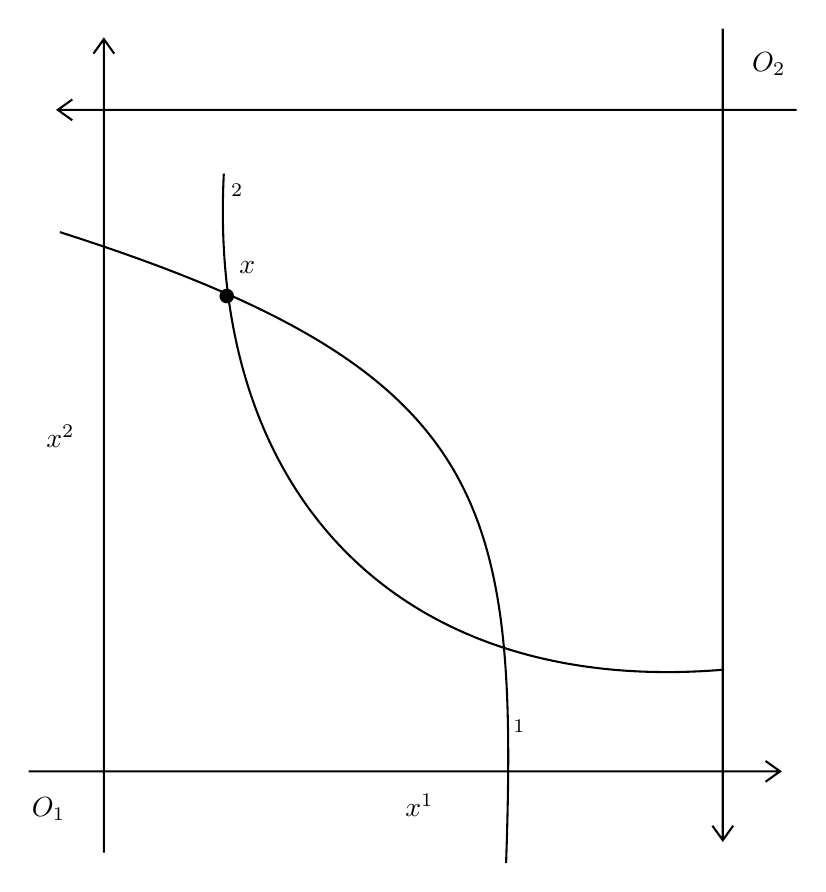
\begin{tikzpicture}[x=0.75pt,y=0.75pt,yscale=-1,xscale=1]
            %uncomment if require: \path (0,484); %set diagram left start at 0, and has height of 484
            %Shape: Axis 2D [id:dp40102790828068324] 
            \draw  (127,388.6) -- (489,388.6)(163.2,35.8) -- (163.2,427.8) (482,383.6) -- (489,388.6) -- (482,393.6) (158.2,42.8) -- (163.2,35.8) -- (168.2,42.8)  ;
            %Shape: Axis 2D [id:dp3759884204481627] 
            \draw  (497,69.9) -- (141,69.9)(461.4,421.8) -- (461.4,30.8) (148,74.9) -- (141,69.9) -- (148,64.9) (466.4,414.8) -- (461.4,421.8) -- (456.4,414.8)  ;
            %Shape: Circle [id:dp6709728610513666] 
            \draw  [fill={rgb, 255:red, 0; green, 0; blue, 0 }  ,fill opacity=1 ] (219.4,159.6) .. controls (219.4,157.94) and (220.74,156.6) .. (222.4,156.6) .. controls (224.06,156.6) and (225.4,157.94) .. (225.4,159.6) .. controls (225.4,161.26) and (224.06,162.6) .. (222.4,162.6) .. controls (220.74,162.6) and (219.4,161.26) .. (219.4,159.6) -- cycle ;
            %Curve Lines [id:da47481039339768105] 
            \draw    (221,100.6) .. controls (213,256.6) and (307,352.6) .. (462,339.6) ;
            %Curve Lines [id:da5885667761847703] 
            \draw    (142,128.8) .. controls (349,194.8) and (363,256.8) .. (357,432.8) ;

            % Text Node
            \draw (127,399.6) node [anchor=north west][inner sep=0.75pt]    {$O_{1}$};
            % Text Node
            \draw (474,40.6) node [anchor=north west][inner sep=0.75pt]    {$O_{2}$};
            % Text Node
            \draw (307,398) node [anchor=north west][inner sep=0.75pt]    {$x^{1}$};
            % Text Node
            \draw (134,220.4) node [anchor=north west][inner sep=0.75pt]    {$x^{2}$};
            % Text Node
            \draw (227,141.4) node [anchor=north west][inner sep=0.75pt]    {$x$};
            % Text Node
            \draw (359,362.4) node [anchor=north west][inner sep=0.75pt]    {$\succsim _{1}$};
            % Text Node
            \draw (223,104) node [anchor=north west][inner sep=0.75pt]    {$\succsim _{2}$};
        \end{tikzpicture}
        \caption{Edgeworth box representing the consumption spaces of individuals 1 and 2.}
        \label{fig:L6-edgeworth-indiff}
    \end{center}
\end{figure}

We assume that preferences are increasing in each good. Therefore, both individuals would like to move away from the origin of their consumption space. As an example, individual \( 1 \) would prefer to be on the dotted indifference curve rather than on the solid one in Figure~\ref{fig:L6-edgeworth-indiff}.

\begin{figure}[H]
    \begin{center}
        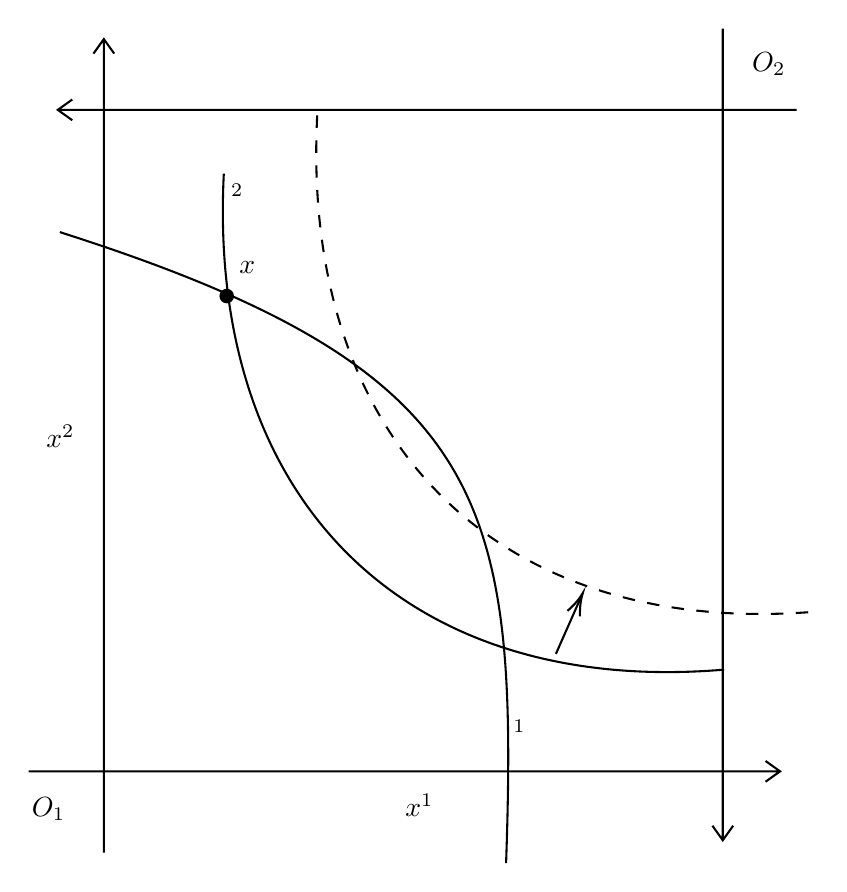
\begin{tikzpicture}[x=0.75pt,y=0.75pt,yscale=-1,xscale=1]
            %uncomment if require: \path (0,484); %set diagram left start at 0, and has height of 484

            %Shape: Axis 2D [id:dp40102790828068324] 
            \draw  (127,388.6) -- (489,388.6)(163.2,35.8) -- (163.2,427.8) (482,383.6) -- (489,388.6) -- (482,393.6) (158.2,42.8) -- (163.2,35.8) -- (168.2,42.8)  ;
            %Shape: Axis 2D [id:dp3759884204481627] 
            \draw  (497,69.9) -- (141,69.9)(461.4,421.8) -- (461.4,30.8) (148,74.9) -- (141,69.9) -- (148,64.9) (466.4,414.8) -- (461.4,421.8) -- (456.4,414.8)  ;
            %Shape: Circle [id:dp6709728610513666] 
            \draw  [fill={rgb, 255:red, 0; green, 0; blue, 0 }  ,fill opacity=1 ] (219.4,159.6) .. controls (219.4,157.94) and (220.74,156.6) .. (222.4,156.6) .. controls (224.06,156.6) and (225.4,157.94) .. (225.4,159.6) .. controls (225.4,161.26) and (224.06,162.6) .. (222.4,162.6) .. controls (220.74,162.6) and (219.4,161.26) .. (219.4,159.6) -- cycle ;
            %Curve Lines [id:da47481039339768105] 
            \draw    (221,100.6) .. controls (213,256.6) and (307,352.6) .. (462,339.6) ;
            %Curve Lines [id:da5885667761847703] 
            \draw    (142,128.8) .. controls (349,194.8) and (363,256.8) .. (357,432.8) ;
            %Curve Lines [id:da5975153383572774] 
            \draw  [dash pattern={on 4.5pt off 4.5pt}]  (266,72.6) .. controls (258,228.6) and (352,324.6) .. (507,311.6) ;
            %Straight Lines [id:da20949155455549462] 
            \draw    (381,332) -- (393.19,304.43) ;
            \draw [shift={(394,302.6)}, rotate = 113.85] [color={rgb, 255:red, 0; green, 0; blue, 0 }  ][line width=0.75]    (10.93,-3.29) .. controls (6.95,-1.4) and (3.31,-0.3) .. (0,0) .. controls (3.31,0.3) and (6.95,1.4) .. (10.93,3.29)   ;

            % Text Node
            \draw (127,399.6) node [anchor=north west][inner sep=0.75pt]    {$O_{1}$};
            % Text Node
            \draw (474,40.6) node [anchor=north west][inner sep=0.75pt]    {$O_{2}$};
            % Text Node
            \draw (307,398) node [anchor=north west][inner sep=0.75pt]    {$x^{1}$};
            % Text Node
            \draw (134,220.4) node [anchor=north west][inner sep=0.75pt]    {$x^{2}$};
            % Text Node
            \draw (227,141.4) node [anchor=north west][inner sep=0.75pt]    {$x$};
            % Text Node
            \draw (359,362.4) node [anchor=north west][inner sep=0.75pt]    {$\succsim _{1}$};
            % Text Node
            \draw (223,104) node [anchor=north west][inner sep=0.75pt]    {$\succsim _{2}$};
        \end{tikzpicture}
        \caption{Individual \( 1 \) would prefer to move on the dotted indifference curve.}
        \label{fig:L6-edgeworth-indiff1}
    \end{center}
\end{figure}

First, we check each individual consumption space, assume monotonic preferences, and draw strictly convex indifference curves.

Then, we introduce prices and budgets, we see the budget set together with the indifference curves, and we discuss the optimum consumption.

We briefly discuss properties of indifference curves.

We introduce endowments for each individual.

Then, we put everything in a single graph, the Edgeworth box. We notice that the individual budget set depends on his endowment and on prices.

We show an instance of budget and demand in which the two preferred allocations are not compatible.

Then, we show a walrasian equilibrium, in which demands are compatible.

We show that when prices are doubled, also wealth is doubled, and the budget set and demand remain the same.

Describe a strange situation in which there are no walrasian equilibria.

Finally, we introduce the concept of Pareto optimality, we show in the Edgeworth box allocations that are and are not Pareto optimal.

Discuss the Pareto set and the contract curve.

Introduce first and second welfare theorems.

Discuss no-envy.

\paragraph{Things to read.} It might be useful for you to review (or study, if you never encountered these topics before), \citet[pp. 51-70, 76-84]{hildenbrandIntroductionEquilibriumAnalysis1976}. If you want (and you \textquote{should want}) to go deeper, study study \citet[pp. 17–23, 40–56]{mas-colellMicroeconomicTheory1995}.

\section{Exercises}

hey.

\bibliographystyle{apacite}  % or another  style
\bibliography{references} % .bib file goes in ./bib/